\documentclass{elektr}
\usepackage{hyperref}
\hypersetup{
colorlinks=true,
urlcolor=blue,
citecolor=blue}
\usepackage[all]{xy,xypic}
\usepackage{amsfonts,amssymb,amsmath,amsgen,amsopn,amsbsy,theorem,graphicx,epsfig}
\usepackage{eufrak,amscd,bezier,latexsym,mathrsfs,eurosym,enumerate}
\usepackage[utf8]{inputenc}\usepackage[english]{babel}
\usepackage{cleveref,multirow}
\usepackage[dvipsnames]{xcolor}
%\usepackage{academicons}
\definecolor{orcidlogocol}{HTML}{A6CE39}
\usepackage[pagewise]{lineno}
\newcommand{\algrule}[1][.2pt]{\par\vskip.5\baselineskip\hrule height #1\par\vskip.5\baselineskip}
\renewcommand{\floatpagefraction}{.9}%
\usepackage{algorithm}
\usepackage[noend]{algpseudocode}
\algnewcommand{\IfThenElse}[3]{
  \State \algorithmicif\ #1\ \algorithmicthen\ #2\ \algorithmicelse\ #3}
\usepackage[font=small,labelfont=bf,tableposition=top]{caption}

\DeclareCaptionLabelFormat{andtable}{#1~#2  \&  \tablename~\thetable}

\linenumbers

\newcommand{\Ab}{\mathbf{A}}
\newcommand{\xb}{\mathbf{x}}
\newcommand{\wb}{\mathbf{w}}
\newcommand{\vb}{\mathbf{v}}

\yil{}
\vol{}
\fpage{}
\lpage{}
\doi{}

\title{Parallel Algorithms for Computing Sparse Matrix Permanents}

\author[Kamer Kaya]{
\textbf{Kamer KAYA\thanks{kaya@sabanciuniv.edu}~\href{https://orcid.org/0000-0001-8678-5467}{\orc}}\\
Computer Science and Engineering, Faculty of Engineering and Natural Sciences, Sabanc{\i} University, Istanbul, Turkey\\
\\ [1.8em]

\rec{.201}
\acc{.201}
\finv{..201}
}

\def\E{\ifmmode{\mathbb E}\else{$\mathbb E$}\fi} %natural numbers
\def\N{\ifmmode{\mathbb N}\else{$\mathbb N$}\fi} %natural numbers
\def\R{\ifmmode{\mathbb R}\else{$\mathbb R$}\fi} %real numbers
\def\Q{\ifmmode{\mathbb Q}\else{$\mathbb Q$}\fi} %rational numbers
\def\C{\ifmmode{\mathbb C}\else{$\mathbb C$}\fi} %complex numbers
\def\H{\ifmmode{\mathbb H}\else{$\mathbb H$}\fi} %complex numbers
\def\Z{\ifmmode{\mathbb Z}\else{$\mathbb Z$}\fi} %integers
\def\P{\ifmmode{\mathbb P}\else{$\mathbb P$}\fi} %real numbers
\def\T{\ifmmode{\mathbb T}\else{$\mathbb T$}\fi} %real numbers
\def\SS{\ifmmode{\mathbb S}\else{$\mathbb S$}\fi} %real numbers
\def\DD{\ifmmode{\mathbb D}\else{$\mathbb D$}\fi} %real numbers

\renewcommand{\a}{\alpha}
\renewcommand{\b}{\beta}
\renewcommand{\d}{\delta}
\newcommand{\D}{\Delta}
\newcommand{\e}{\epsilon}
\newcommand{\var}{\varepsilon}
\newcommand{\g}{\gamma}
\newcommand{\la}{\lambda}
\newcommand{\La}{\Lambda}
\newcommand{\lan}{\langle}
\newcommand{\ran}{\rangle}
\newcommand{\n}{\nabla}
\newcommand{\va}{\varphi}
\newcommand{\s}{\sigma}
\newcommand{\Sig}{\Sigma}
\renewcommand{\t}{\tau}
\renewcommand{\th}{\theta}
\newcommand{\Om}{\Omega}
\newcommand{\om}{\omega}
\newcommand{\pa}{\partial}
\newcommand{\up}{\upsilon}
\newcommand{\vp}{\varphi}
\newcommand{\z}{\zeta}





\newcommand{\bse}{\begin{subequations}}
\newcommand{\ese}{\end{subequations}}
\newcommand{\ben}{\begin{enumerate}}
\newcommand{\een}{\end{enumerate}}
\newcommand{\bens}{\begin{enumerate*}}
\newcommand{\eens}{\end{enumerate*}}
\newcommand{\be}{\begin{equation}}
\newcommand{\ee}{\end{equation}}
\newcommand{\bea}{\begin{eqnarray}}
\newcommand{\eea}{\end{eqnarray}}
\newcommand{\baa}{\begin{eqnarray*}}
\newcommand{\eaa}{\end{eqnarray*}}
\newcommand{\bc}{\begin{center}}
\newcommand{\ec}{\end{center}}
\newcommand{\ol}{\overline}
\newcommand{\ul}{\underline}
\newcommand{\ov}{\overbrace}
\newcommand{\uv}{\underbrace}
\newcommand{\Ra}{\Rightarrow}
\newcommand{\ra}{\rightarrow}
\newcommand{\ds}{\displaystyle}
\newcommand{\vs}{\vspace}


\newcommand{\IR}{\mbox{I \hspace{-0.2cm}R}}
\newcommand{\IN}{\mbox{I \hspace{-0.2cm}N}}



%% \theoremstyle{plain} %% This is the default

\newtheorem{theorem}{Theorem}%[section]

\theoremstyle{corollary}
\newtheorem{corollary}{Corollary}

\theoremstyle{lemma}
\newtheorem{lemma}{Lemma}

\theoremstyle{proposition}
\newtheorem{proposition}{Proposition}

\theoremstyle{axiom}
\newtheorem{axiom}{Axiom}

\theoremstyle{conjecture}
\newtheorem{conjecture}{Conjecture}

\theoremstyle{example}
\newtheorem{example}{Example}

\theoremstyle{definition}
\newtheorem{definition}{Definition}%[section]

\theoremstyle{remark}
\newtheorem{remark}{Remark}%[section]
\newtheorem{notation}{Notation}


\newtheorem{question}{Question}%[section]
\newtheorem{construction}{Construction}

\newtheorem{athm}{Theorem}
\renewcommand{\theathm}{\Alph{athm}}



\setcounter{page}{1}
\begin{document}

\maketitle


\begin{abstract}
The permanent is an important characteristic of matrices and it has been used in many applications in both theory and practice. Although its definition is simple, it is a hard to compute immanant. For dense and/or full matrices, the fastest exact algorithm at hand has $\mathcal{O}(2^{n-1}n)$ complexity. However, for sparse matrices, there are various techniques that can be applied to improve the practical performance. In this work, we propose the algorithm {\sc{SkipPer}} that uses a technique to exploit the sparsity of the matrix as much as possible, restructure the matrix to reduce the overall work, and enable coarse-grain, shared-memory parallelization with dynamic scheduling. Our experiments show that {\sc{SkipPer}} increases the performance of exact permanent computation up to $140\times$ compared to the naive version proposed for full matrices. Furthermore, thanks to the coarse-grain parallelization, we obtain $14$--$15\times$ speedup on average with $\tau = 16$ threads over the sequential algorithm. Overall, by exploiting the sparsity and parallelism, the speedup is $2000\times$ for some of the matrices we used in our experimental setting.   
\keywords{Sparse matrices, permanent, Ryser's algorithm, multicore CPUs, shared-memory parallelism, load balancing.}
\end{abstract}

\section{Introduction}\label{Int}
Given an $n \times n$ matrix $\Ab$ with entries $a_{i,j}$ for $1 \leq i,j \leq n$, the permanent is computed as 
\begin{equation}
{\tt perm}(\Ab) = \sum_{\sigma \in {\mathcal P}}{\prod_{i=1}^{n}a_{i, \sigma(i)}} \label{eq1}
\end{equation}
where ${\mathcal P}$ is the set of all permutations of the numbers in $\{1, 2, \cdots, n\}$. As an immanant, it is mainly of interest due to its applications in number theory~(e.g.,~\cite{kilic07}) and probability theory and statistics~(e.g.,~\cite{balakrishnan07}).  
Permanents also have found applications in Quantum Computing~\cite{aaronson11} and even in Bioinformatics~\cite{narahara13}. 
Furthermore, it has interesting relations with graph theory; with an efficient algorithm to compute ${\tt perm}(\Ab)$, one can count the number of perfect matchings for a bipartite graph or find the number of vertex-disjoint cycle covers of a directed graph. These two statements are direct conclusions of~\eqref{eq1} when a (0,1)-matrix $\Ab$ is generated as the bi-adjacency or adjacency matrix, respectively. More applications of the permanents and their relations with theory and practice can be found in~\cite{minc84}.
Unfortunately, computing the permanent of a (0,1)-matrix is \#P-complete~\cite{valiant79} and there exist studies in the literature on approximating the permanent~(e.g.,~\cite{dufosse18}).  

There exist various studies focusing on the exact computation of~\eqref{eq1}, especially when the matrix is sparse~\cite{mittal01, servedio05, bax08, yue13}. To the best of our knowledge, when the matrix is dense/full, Ryser's algorithm from 1963 is still the most efficient algorithm at hand~\cite{ryser63}. It uses the inclusion/exclusion principle and compute the permanent with $\mathcal{O}(2^{n-1}n^2)$ time complexity. Later, Niejenhuis and Wilf proposed to process the sets in Gray-code order to reduce the complexity to $\mathcal{O}(2^{n-1}n)$~\cite{nijenhuis78}. 

In this work, we focus on computing the permanents of sparse matrices in parallel and propose novel algorithms based on the Niejenhuis-Wilf variant of the Ryser's algorithm. When the matrix is sparse, various optimizations can be applied; for instance, when the number of possible transversals, i.e., sets of $n$ nonzero matrix entries such that no two come from the same row or the same column, is small, one can enumerate all the transversals and sum their contributions to the permanent. Unfortunately, this is not the case for many matrices. As we will show in this work, even when the number of transversals is large, depending on the level of sparsity, one can incur optimizations that yield a shorter permanent computation time. Furthermore, although the Gray-code order seem to necessitate inherently sequential iterations, with a slight modification on Ryser's original approach, one can parallelize the execution flow and assign a balanced work load to the threads via dynamic scheduling. 

The rest of the paper is organized as follows: Section~\ref{sec:back} presents the Ryser's algorithm and related work. Section~\ref{sec:spa} describes the basic approach to exploit the sparsity. A further optimization that focuses on skipping the zero-contributing gray codes and a coarse-grain parallelization technique is described in Section~\ref{sec:skip}. The related literature is summarized in Section~\ref{sec:rel}. Section~\ref{sec:exp} presents the results of the experiments and Section~\ref{sec:conc} concludes the paper.  

\section{Background and Notation}\label{sec:back}

For an $n \times n$ matrix, Eq.~\ref{eq1} defines the permanent in terms of transversals. With a naive algorithm, computing the total contribution of all transversals takes $\mathcal{O}(n \times n!)$ time. To reduce the complexity, Ryser's algorithm restructures the original permanent equation and performs inclusion/exclusion as follows
\begin{equation}
{\tt perm}(\Ab) = -1^n  \sum_{S \subseteq \{1,2, \cdots, n\}} (-1)^{|S|} \prod_{i=1}^{n} \sum_{j \in S}{a_{i,j}} \label{eq2}
\end{equation}
The pseudocode of the Niejenhuis-Wilf variant of Ryser's algorithm, {\sc{Ryser}}, is given in Algorithm~\ref{alg:ryser}. In the pseudocode, {\sc{Gray}}$_{g}$ is the $g$th Gray code with $(n-1)$ bits; a 4-bit Gray code is shown on the right of the algorithm. For a binary-reflected Gray code, $$\mbox{\sc{Gray}}_{g} = g \oplus (g \gg 1)$$ where $\oplus$ is the bitwise XOR operation and $g \gg 1$ shifts the bitwise representation of $g$ to the right by one bit.  

Let {\sc{Gray}}$_{g}$[$j$] be the $j$th bit of  {\sc{Gray}}$_{g}$ where $j = 1$ denotes the least significant bit. The set bits, i.e., the ones equal to $1$, for each code represent the indices of the selected columns. To store and keep the impact of these columns, the algorithm keeps maintaining a vector $\xb$, whose $i$th entry relates to the contribution of the $i$th row of the matrix. For each $g$, the algorithm first finds the difference between {\sc{Gray}}$_{g}$ and {\sc{Gray}}$_{g-1}$, i.e., the changed bit in {\sc{Gray}}$_{g}$~(line~\ref{ln:j}). Then the updates due to this bit modification are performed on $\xb$~(line~\ref{ln:xb}). Finally, the product of these vector entries is added to $p$~(line~\ref{ln:p}). Note that the Niejenhuis-Wilf variant practically uses an $(n-1)$-bit Gray code, not an $n$-bit one, for an $n \times n$ matrix to halve the execution time. 

\begin{minipage}{0.5\textwidth}
\begin{center}
\begin{algorithm}[H]
\caption{: {\sc Ryser}} \label{alg:ryser}
 \hspace*{\algorithmicindent} \textbf{Input:}  \hspace*{1.5ex}$\Ab$~($n \times n$ matrix) \\
 \hspace*{\algorithmicindent} \textbf{Output:} {\tt perm}($\Ab$)
 \algrule
\begin{algorithmic}[1]

\For{$i = 1$ to $n$} 
	\State{$sum = 0$}
	\For{$j = 1$ to $n$} 
		\State{$sum \leftarrow sum + a_{i,j}$}
	\EndFor
	\State{$\xb \leftarrow a_{i,n} - \frac{sum}{2}$}	
\EndFor
 \algrule

\State{$p \leftarrow \prod_{i = 1}^n{\xb[i]}$}

 \algrule

 \For {$g = 1$ to $2^{n-1} - 1$} \label{ln:loop1}
	\State{$j \leftarrow \log_2$({\sc{Gray}}$_{g}$ $\oplus$ {\sc{Gray}}$_{g-1}$)}\label{ln:j}
	\State{$s \leftarrow 2 \times ${\sc{Gray}}$_{g}$[$j$] $-1$}
	 \State{$prod \leftarrow 1$}
	 \For {$i =  1$ to $n$} \label{ln:loop2}
	        \State{$\xb[i] \leftarrow \xb[i] + (s \times a_{i, j})$}\label{ln:xb}
	        \State{$prod \leftarrow prod \times \xb[i]$}	        
	 \EndFor

	 \State{$p \leftarrow p + \left((-1)^g \times prod\right)$}\label{ln:p}
\EndFor 
	  \algrule

\State{\Return{$p \times (4 \times (n \bmod 2) - 2)$}}
 \end{algorithmic}
\end{algorithm}
\end{center}
\end{minipage}
\hspace*{10ex}
\begin{minipage}{0.3\textwidth}
\scalebox{0.95}{
\begin{tabular}{lll}
&	{\sc{Binary}}	&{\sc{Gray}}\\\hline
{\sc{Gray}}$_{0}$	&0000	&0000\\
{\sc{Gray}}$_{1}$	&0001	&0001\\
{\sc{Gray}}$_{2}$	&0010	&0011\\
{\sc{Gray}}$_{3}$	&0011	&0010\\
{\sc{Gray}}$_{4}$	&0100	&0110\\
{\sc{Gray}}$_{5}$	&0101	&0111\\
{\sc{Gray}}$_{6}$	&0110	&0101\\
{\sc{Gray}}$_{7}$	&0111	&0100\\
{\sc{Gray}}$_{8}$	&1000	&1100\\
{\sc{Gray}}$_{9}$	&1001	&1101\\
{\sc{Gray}}$_{10}$	&1010	&1111\\
{\sc{Gray}}$_{11}$	&1011	&1110\\
{\sc{Gray}}$_{12}$	&1100	&1010\\
{\sc{Gray}}$_{13}$	&1101	&1011\\
{\sc{Gray}}$_{14}$	&1110	&1001\\
{\sc{Gray}}$_{15}$	&1111	&1000\\
\end{tabular}
}
\end{minipage}

To the best of our knowledge, Ryser's algorithm is currently the most efficient one for the exact computation of permanents of generic, dense matrices. In the pseudocode above, the outer loop~(line~\ref{ln:loop1}) iterates exactly $(2^{n-1}-1)$ times and the inner loop~(line~\ref{ln:loop2}) iterates $n$ times. Hence, the overall complexity is $\mathcal{O}(2^{n-1}n)$.

\begin{figure}[H]
\begin{center}
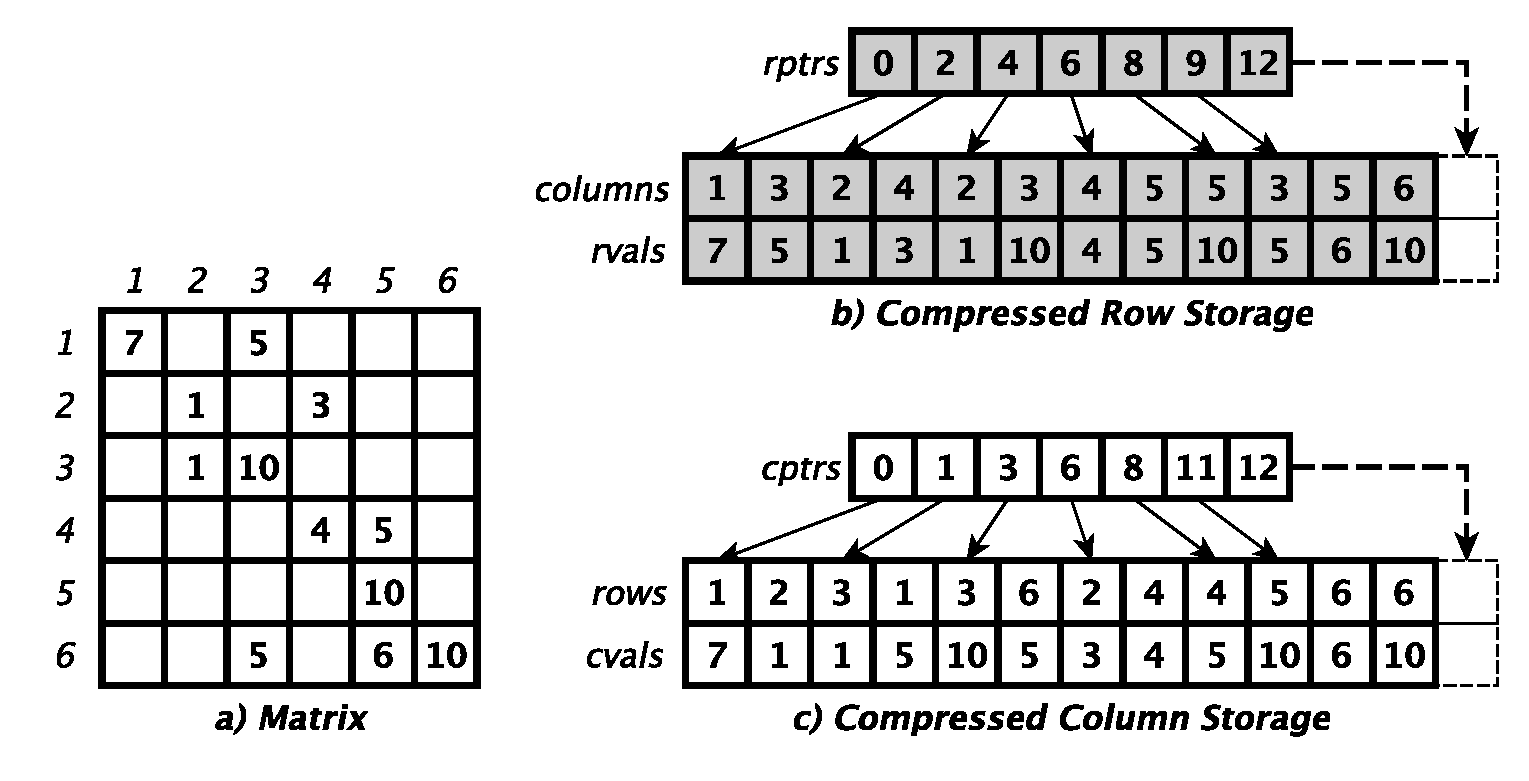
\includegraphics[width=0.7\linewidth]{fig1.pdf}
\caption{({\bf a}) A $6 \times 6$ matrix and its ({\bf b}) CRS and ({\bf c}) CCS representations.}
\label{fig:mat}
\end{center}
\end{figure}

\section{{\sc{SpaRyser}}: An Algorithm for Sparse Permanents} \label{sec:spa}

A sparse matrix has many zero entries; for permanents, as well as for {\sc{Ryser}}, such entries do not have a practical impact on the final value since, when the selected traversal contains a single zero, its whole contribution becomes zero. Hence, such entries can be removed from the matrix and the remaining part can be stored with an appropriate data structure. The most widely used sparse-matrix data structures in the literature are {\em Compressed Row/Column Storage}~(CRS and CCS). To store the sparse nonzero pattern, these structures uses two arrays where the entries of the first one denotes the start locations of each sparse row/column whose column/row ids are consecutively stored in the second array. An additional array, whose index structure is the same as the second array, is used to store the nonzero values. A toy matrix and its CRS/CCS representations are given in Figure~\ref{fig:mat}. Using such a structure for permanent computation has been proposed by Mittal and Al-Kurdi~\cite{mittal01}. However, their approach computes the permanent via enumeration and can be used only for matrices when the number of all transversals is small. That is their algorithm is based on~\eqref{eq1} whereas the proposed algorithms {\sc SpaRyser} and {\sc SkipPer} in this work  are based on~\eqref{eq2}. 

\begin{algorithm}[htbp]
\caption{: {\sc SpaRyser}} \label{alg:sparyser}
 \hspace*{\algorithmicindent} \textbf{Input:}  \hspace*{1ex} ($rptrs,  columns, rvals$) - CRS of $\Ab$ \\ \hspace*{14.3ex}($cptrs, rows,  \hspace*{3.6ex}cvals$) - CCS of $\Ab$\\
 \hspace*{\algorithmicindent} \textbf{Output:} {\tt perm}($\Ab$)

\algrule
\begin{algorithmic}[1]

\State{$nzeros \leftarrow 0$}
\For{$i = 1$ to $n$} 
	\State{$sum = 0$}
	\For{$ptr = rptrs[i]$ to ($rptrs[i+1] - 1$)} 
		\State{$sum \leftarrow sum + rvals[ptr]$}
	\EndFor
	\State{$\xb[i] \leftarrow rvals[rptrs[i+1] - 1]- \frac{sum}{2}$}	
	\If{$\xb[i] = 0$}
		\State{$nzeros \leftarrow nzeros + 1$}
	\EndIf
\EndFor

 \algrule
\If{$nzeros > 0$}
	\State{$p \leftarrow \prod_{i = 1}^n{\xb[i]}$}
\Else
	\State{$p \leftarrow 0$}
\EndIf


 \algrule
 \For {$g = 1$ to $2^{n-1} - 1$} \label{ln:loop1spa}
	\State{$j \leftarrow \log_2$({\sc{Gray}}$_{g}$ $\oplus$ {\sc{Gray}}$_{g-1}$)}
	\State{$s \leftarrow 2 \times ${\sc{Gray}}$_{g}$[$j$] $-1$}	 
	  \For {$ptr = cptrs[j]$ to ($cptrs[j + 1] - 1$)}
	        \State{$row \leftarrow rows[ptr]$}
	        \State{$val \leftarrow cvals[ptr]$}

	        \If{$\xb[row]  = 0$}
	        	\State{$nzeros \leftarrow nzeros - 1$}
	        \EndIf
	        \State{$\xb[row] \leftarrow \xb[row] + (s \times val)$}\label{ln:xbspa}
	         \If{$\xb[row]  = 0$}
	        	\State{$nzeros \leftarrow nzeros + 1$}
	        \EndIf
	 \EndFor

	 \If{$nzeros = 0$}
	 	\State{$prod \leftarrow 1$}
	 	\For {$i =  1$ to $n$} 
	        		\State{$prod \leftarrow prod \times \xb[i]$}	        
	 	\EndFor
		\State{$p \leftarrow p + \left((-1)^g \times prod\right)$}
	\EndIf
\EndFor 

\algrule
\State{\Return{$p \times (4 \times (n \bmod 2) - 2)$}}
 \end{algorithmic}
\end{algorithm}


For a dense/full matrix, regardless of the flipped bit, there will be $n$ updates on the vector $\xb$. However, for a sparse matrix, one can exploit the sparsity with CCS representation, since the zero entries, which have zero contribution on the $\xb$ vector, can be skipped. Thanks to CCS, when the $j$th bit is flipped in the Gray code, the number of updates to the vector will exactly be equal to the number of nonzero elements on column $j$. 
Note that {\sc Ryser} also performs the same number of useful updates; but it also performs updates with no impact. 
Hence, in terms of the number of floating point operations, using CRS and CCS can significantly increase the efficiency based on the level of sparsity in the matrix. The pseudocode of {\sc{SpaRyser}} is given in Algorithm~\ref{alg:sparyser}.

In addition to the exploitation of sparsity, {\sc{SpaRyser}} performs two other techniques for fast permanent computation: 
\begin{enumerate}
\item In Algorithm~\ref{alg:ryser}, {\sc Ryser}, the inner loop~(at line~\ref{ln:loop2}) has two statements. Using CRS and CCS in {\sc SpaRyser} only reduces the number of $\xb$ updates on the first line but the $\Theta(n)$ cost of the second line to compute $prod$ is still there. Our preliminary experiments showed that for a significant number of iterations of the main loop, i.e., for many $g$ values, the contribution, and hence the value of the $prod$, can be zero in sparse matrices. However, even for these $g$ values, {\sc Ryser} performs all the multiplications. To get rid of these unnecessary operations, {\sc{SpaRyser}} counts the number of zeros with a variable $nzeros$ and when a zero is detected, i.e., when $nzeros$ is positive, it does not compute the product and does not update $p$.   
\item Both {\sc{Ryser}} and {\sc{SpaRyser}} use a binary-reflected Gray code. For an $n$-bit, binary-reflected Gray code, the $j$th bit changes $2^{n - j}$ times for $1 \leq j \leq n$. Hence, there is a significant imbalance on the numbers of bit flips for different bit locations. Such an imbalance yields an avenue for further optimization. To increase the performance of the algorithm, we apply a preprocessing step and order the columns in increasing number of nonzeros. This ordering is expected to increase the performance, since sparser columns are processed more frequently when compared to the denser ones. Clearly, the amount of improvement depends on the imbalance on the number of column nonzeros. We call this ordering scheme {\sc{SortOrd}}.
\end{enumerate}

\section{{\sc{SkipPer}}: Faster Sparse Permanents with Gray Skipping and Parallelization} \label{sec:skip}

With {\sc{SpaRyser}}, the sparsity is exploited and the unnecessary multiplications are omitted. However, one can further avoid them by explicitly skipping these iterations, which will yield even a faster algorithm. That is, instead of checking a zero vector-product for every iteration, when a zero-contributing Gray code is detected, one can skip as many iterations as possible with a single jump. Nevertheless, the jumps must not skip a contributing iteration. To jump as long as possible, the proposed algorithm {{\sc{SkipPer}} uses the following lemma. 
\begin{lemma} 
In an $n$-bit binary-reflected Gray code, the value of the $j$th bit of {\sc{Gray}}$_{g}$, for $1 \leq j \leq n$, is
\[
  \mbox{{\sc{Gray}}}_{g}[j] =
  \begin{cases}
                                   0 & \text{if $g < 2^{j-1}$} \\
                                   \left(\lfloor \frac{(g - 2^{j-1})}{2^{j}}\rfloor \bmod 2\right) + 1& \text{otherwise} 
  \end{cases}
\]
\label{lem:gray}
\end{lemma}
The lemma is exploited as follows; when a zero entry $\xb[i]$ is detected throughout the execution, at least one of the columns of $\Ab$ having a nonzero at its $i$th position needs to be processed to make  $\xb[i]$ nonzero. In Ryser's approach, a column is processed when the corresponding bit in the Gray code changes. Let $next(g, j)$ be the first iteration after $g$th iteration where {\sc{Gray}}$_{g}[j] \neq ${\sc{Gray}}$_{next(g, j)}[j]$ for $1 \leq j \leq n$. Based on the lemma, this iteration can be computed as:
$$next(g, j) = 
 \begin{cases}
2^j & \text{if $g < 2^j$} \\
g + 2^{j+1} - ((g-2^j) \bmod (2^{j + 1}))& \text{otherwise}
\end{cases}
$$
For completeness, we need to state that in an $n$-bit Gray code, when $next(g, j) \geq 2^n$, {\sc{Gray}}$_{g}[j]$ is already the last value for $j$th bit and it will never be changed. 

Using $next(g, j)$, for a vector entry $\xb[i] = 0$ encountered at iteration $g$, {{\sc{SkipPer}} computes 
$$g^{(i)} = \min{\{next(g, j): a_{i,j} \neq 0\}}$$
to find the earliest iteration that can make $\xb[i] \neq 0$. Hence, assuming $\xb$ is the current vector at iteration $g$, the first iteration that can produce a nonzero $prod$ value is 
$$next(g) = 
 \begin{cases}
g+1 & \text{if $\xb[i] \neq 0,\ \text{ for } 1 \leq i \leq n$} \\
\max\{g^{(i)}: \xb[i] = 0\}$$& \text{otherwise}
\end{cases}
$$

\algrenewcommand\algorithmicindent{1.0em}%
\begin{minipage}[t]{0.48\textwidth}
\begin{algorithm}[H]
\caption{: {\sc SkipPer}} \label{alg:skipper}
 \hspace*{\algorithmicindent} \textbf{Input:}   \hspace*{2ex}($rptrs, columns, rvals$) - CRS of $\Ab$ \\ \hspace*{13.3ex}($cptrs, rows, \hspace*{3.6ex}cvals$) - CCS of $\Ab$\\
 \hspace*{\algorithmicindent} \textbf{Output:} {\tt perm}($\Ab$)

\algrule
\begin{algorithmic}[1]

\For{$i = 1$ to $n$} 
	\State{$sum = 0$}
	\For{$ptr = rptrs[i]$ to ($rptrs[i+1] - 1$)} 
		\State{$sum \leftarrow sum + rvals[ptr]$}
	\EndFor
	\State{$\xb[i] \leftarrow rvals[rptrs[i+1] - 1]- \frac{sum}{2}$} \label{ln:x}
\EndFor

 \algrule
\State{$p \leftarrow \prod_{i = 1}^n{\xb[i]}$}
\State{$g' \leftarrow 0$}
\State{$g \leftarrow 1$}
 \algrule
 \While{$g < 2^{n - 1}$} \label{ln:loop1jmp}
	 \State{$gr_{diff} = g \oplus g'$}	\label{ln:skp1}	
	  \For{$j = 1$ to $n$}  \label{ln:loop2jmp}
	  \If{$gr_{diff}[j] = 1$}
	  \State{$gr_{diff}[j] \leftarrow 0$}
	  \State{$s \leftarrow 2 \times ${\sc{Gray}}$_{g}$[$j$] $-1$}
 	  \For {$ptr = cptrs[j]$ to $cptrs[j + 1] - 1$}
	        \State{$row \leftarrow rows[ptr]$}
	        \State{$val \leftarrow cvals[ptr]$}
	        \State{$\xb[row] \leftarrow \xb[row] + (s \times val)$}\label{ln:skp2}
	       \EndFor
	 \EndIf
	 \EndFor 

	 	\State{$prod \leftarrow 1$}
	 	\For {$i = 1$ to $n$} \label{ln:loop2spa}
	        		\State{$prod \leftarrow prod \times \xb[i]$}	        
	 	\EndFor
		\State{$p \leftarrow p + \left((-1)^g \times prod\right)$}
 \algrule
	\State{$g' \leftarrow g$}
	\State{$g \leftarrow next(g)$}
	\EndWhile 

\algrule
\State{\Return{$p \times (4 \times (n \bmod 2) - 2)$}}
 \end{algorithmic}
\end{algorithm}
\end{minipage}
\hspace*{3ex}
\begin{minipage}[t]{0.4\textwidth}
\begin{algorithm}[H]
\caption{: {\sc SkipOrd}} \label{alg:order}
 \hspace*{\algorithmicindent} \textbf{Input:} \hspace*{1.1ex}  $\Ab$~($n \times n$ matrix)\\
 \hspace*{\algorithmicindent} \textbf{Output:} $\Ab'$~(row/col permuted $\Ab$)
\algrule
\begin{algorithmic}[1]
\State{$rowPerm \leftarrow [.]$}
\State{$colPerm \leftarrow [.]$}
\State{$rowVisited \leftarrow [.]$}
\State{$degs \leftarrow [.]$}
\For{$j = 1$ to $n$} 
	\State{$degs[j] \leftarrow 0$}
	\State{$rowVisited[j] \leftarrow {\bf false}$}
\EndFor

\For{$i = 1$ to $n$}
	\For{$j = 1$ to $n$} 
		\If{$a_{i, j} \neq 0$}  
			\State{$degs[j] \leftarrow degs[j]  + 1$}
		\EndIf
	\EndFor
\EndFor

\State{$i \leftarrow 1$}
\For{$j = 1$ to $n$} 
\State{$curCol \leftarrow \underset{\ell}{argmin} \{degs[\ell]\}$} \label{order:col}
\State{$degs[curCol] \leftarrow \infty$}\label{ln:order}
\State{$colPerm[j] \leftarrow curCol$}
\For{all $\ell$ s.t. $a_{\ell, curCol} \neq 0$} \label{order:row}
\If{$rowVisited[\ell] = {\bf false}$}
\State{$rowVisited[\ell] \leftarrow {\bf true}$}
\State{$rowPerm[i] \leftarrow \ell$}
\State{$i \leftarrow i + 1$}

\For{all $k$ s.t. $a_{\ell, k} \neq 0$}
	\If{$degs[k] \neq \infty$}
		\State{$degs[k] \leftarrow degs[k] - 1$} \label{order:row2}

	\EndIf
\EndFor
\EndIf
\EndFor
\EndFor
\State{$\Ab' \leftarrow \Ab[rowPerm, colPerm]$}
\end{algorithmic}
\end{algorithm}
\end{minipage}

It is indeed safe to jump from iteration $g$ to $next(g)$ for each $1 \leq g < 2^{n-1} - 1$ since all nonzero contributions of all the iterations will still be taken into account. Yet, we also need an efficient mechanism to find the entries in vector $\xb$ at iteration $next(g)$; we only have $\xb$ for iteration $g$ and not for the iterations in between. Fortunately, this can be efficiently done by computing the bitwise difference of {\sc{Gray}}$_{g}$ and {\sc{Gray}}$_{next(g)}$ as Algorithm~\ref{alg:skipper} shows~(lines~\ref{ln:skp1}--\ref{ln:skp2}). 


By using the $next(.)$ function, {\sc SkipPer} skips the zero-contributing transversals as much as possible. To increase the length of skips, we employ an ordering as a preprocessing step whose pseudocode is shown in Algorithm~\ref{alg:order}}. As described in the previous section, the ordering technique in {\sc{SpaRyser}} was sorting the columns based on
their number of nonzeros. 
For {\sc SkipPer}, we use a similar, sorting-like column ordering,  {\sc SkipOrd}, which dynamically updates the degree counts~($degs$ in the pseudocode) after each column selection in a way that the degree of each 
unselected column is always equal to the number of its rows that are not yet touched by previously chosen columns. That is $degs[j]$ is the additional number of rows touched for the first time if column $j$ is chosen. Throughout the process, we always continue with the column having minimum $degs$ value~(line~\ref{order:col}).  To ignore already chosen columns during this selection, we immediately set $degs[j] \leftarrow \infty$ once column $j$ is selected~(line~\ref{ln:order} of Algorithm~\ref{alg:order}). 

In {\sc SkipOrd}, we track the steps where the rows are touched for the first time; unlike {\sc{SortOrd}}, this yields a row ordering which is integrated to the process~(lines~\ref{order:row}--\ref{order:row2} Algorithm~\ref{alg:order}). Such a row ordering creates a structure with entries close to the diagonal in the lower triangular part of the matrix. This is expected to increase the performance; when a vector entry $\xb[i] = 0$ with a large $i$~(close to $n$) is encountered, to increase the length of the jumps, we want $\xb[i]$ to keep its value as long as possible. Since the Gray-code is unbalanced and the later bits are less frequently flipped, $\xb[i]$ will be zero for a long time if flipping the earlier bits do not yield an update on $\xb[i]$. This is what the row-ordering in {\sc{SkipOrd}} provides and this is why this ordering is expected to make {\sc{SkipPer}} faster. 

\subsection{Parallel Permanent Computation with {\sc{SkipPer}}} \label{sec:par}

As Algorithm~\ref{alg:skipper} shows, there are loop workloads at two levels where the size of the iteration space is $2^{n-1} - 1$ for the first level~(line~\ref{ln:loop1jmp}) and $n$ for the second level~(lines \ref{ln:loop2jmp} and~\ref{ln:loop2spa}). Since $2^{n-1}$ much larger than $n$ and a coarse-grain parallelism usually creates less overhead, it is better to divide the permanent computation into a number of tasks through the outer loop.  Hence, the threads will process different iterations, i.e., different chunks of consecutive Gray codes. Although it seems hard to start processing arbitrary chunks at first look, by using the technique in {\sc SkipPer}, the threads can skip all the iterations until the first iteration of any chunk. Hence, the previous approach can be used to divide all the iteration space to $\tau$ threads.  

Let $t_i$ be the $i$th thread for $1 \leq i \leq \tau$. To parallelize {\sc{SkipPer}}, one can simply divide the iteration space into equisized chunks of size $c = \lfloor 2^{n-1} - 1) / \tau \rfloor$~(the last thread may perform a few more iterations if $\tau$ does not divide $2^{n-1}$). Each thread computes the first iteration of its chunk by computing $g^i_{first} = c \times (i-1) + 1$ and process the Gray codes in the iteration space $[g^i_{first}, g^{i+1}_{first})$ where for completeness, $g^{\tau+1}_{first} =  2^{n-1}$. The $\xb$ vector~(as computed in line~\ref{ln:x} of Algorithm~\ref{alg:skipper}) is copied to the private memory of each thread and the private copy $\xb^i$ is updated based on $g^i_{first}$ by $t_i$. After the initialization step, the threads process their chunks as in the sequential {\sc SkipPer}. Since the parallelized variant is quite similar, here we do not provide a pseudocode. 

One problem with this simple approach using static scheduling is that although each iteration seem to be equal in terms of its computational load, especially for sparse matrices, an unexpected number of iterations are skipped in a single chunk. Since the number of skipped iterations can greatly vary for different chunks,  when static scheduling is used, the workload distribution among the threads can be highly irregular. To better balance the loads, once can use more, smaller chunks and assign the chunks to the idle threads one by one throughout the execution, i.e., perform dynamic scheduling. 

\section{Related Work}\label{sec:rel}

There are a few studies on computing exact permanents for sparse matrices: Mittal and Al-Kurdi proposed an algorithm which  enumerates all the permanents by exploiting the efficiency of CRS and CCS representations~\cite{mittal01}. Their algorithm is efficient for very sparse matrices with a small number of transversals. When the number of transversals is large, which is usually the case in practice, the execution time increases significantly. Computing permanents of special matrix classes, e.g., ($0$-$1$)-matrices, have been also investigated in the literature~\cite{bax08}.

Forbert and Marx proposed an approximation algorithm for sparse permanents~\cite{forbert03}. In the same study, they also presented a decomposition scheme based on the following equation:
\begin{equation}
{\tt perm}
\left(
\begin{bmatrix}
    a    & b& \mathbf{c} \\
  \mathbf{d}      & \mathbf{e} & \mathbf{A'} 
\end{bmatrix}
\right)
=
{\tt perm}
\left(\begin{bmatrix}
     0   & 0& \mathbf{c} \\
  \mathbf{d}      & \mathbf{e} & \mathbf{A'}
  \end{bmatrix}
\right)
+
{\tt perm}
\left(
\begin{bmatrix}
    a\mathbf{e}  + b\mathbf{d}  & \mathbf{A'} 
    \end{bmatrix}
\right)
\label{eq:expand}
\end{equation}
where for an $n \times n$ input matrix on the left side of equality, $a$ and $b$ are scalars, $\mathbf{c}$ is an ($n-2$)-dimensional row
vector, $\mathbf{d}$ and $\mathbf{e}$ are ($n-1$)-dimensional column vectors, and $\mathbf{A'}$ is the ($n - 1$) $\times$ ($n - 2$)  left over matrix. 
This decomposition scheme is exploited by Liang~et~al.~\cite{liang06} and a hybrid algorithm is proposed which
recursively decomposes the matrices via~\eqref{eq:expand} if there exists a row/column with less than or equal to four nonzeros. If this is
not the case, i.e., when all the rows/columns have more than four nonzeros, the algorithm calls {\sc{Ryser}}. The proposed algorithms
in this study, especially {\sc{SkipPer}}, can be used instead of {\sc{Ryser}} in this hybrid algorithm. 

The experiments of Liang~et~al. show that when the density of the matrix, i.e., the ratio of the number of nonzeros to $n^2$, is $40\%$, the execution times of the proposed hybrid algorithm
and {\sc{Ryser}} is comparable. They also reported that for a $25 \times 25$ matrix having $25\%$ density, the execution time ratio of 
{\sc{Ryser}} and the hybrid algorithm is $1.5$. 
As the next section will show, {\sc{Skipper}} alone, even without decomposition, provides much
better speedups especially when the sparsity is higher. Note that as $n$ increases with a constant sparsity, the decomposition technique becomes less and less effective 
since the expected number of nonzeros on a row/column increases and becomes more than four. 
The hybrid algorithm in~\cite{liang06} was also used by Yue~et~al.~\cite{yue13} where the matrix is first partitioned into two for a more
efficient permanent computation. Similar to aforementioned studies, the proposed 
algorithms in this paper can be used instead of the hybrid algorithm, or inside the hybrid algorithm, to improve the performance.  

Since the decomposition can yield many matrices, a trivial parallelization strategy would be assigning all the final sub-matrices to a different thread/processor/node etc. 
This strategy is considered in~\cite{Wang2012ALB} with a load-balancing technique based on estimating the hardness of the permanent computation for each sub-matrix. Similar to above, if decomposition 
is not applicable, one cannot divide the task into sub-tasks with this strategy. However, even if this is the case, the proposed parallelization of {\sc{Skipper}} can be employed. Furthermore, as the experiments will show,
with dynamic scheduling this strategy yields almost linear speedups hence it can be used without hesitation even when decomposition is possible.

\section{Experimental Results}\label{sec:exp}

To analyze the performance of {\sc{Ryser}}, {\sc{SpaRyser}} and {\sc{SkipPer}} and measure the performance improvements obtained due to exploitation of sparsity, Gray skipping and parallelization, we conduct experiments on   synthetic and real-life matrices. All the experiments are performed on a server running on 64-bit CentOS 6.5 equipped with 64GB RAM and two
Intel Xeon E7-4870 v2 clocked at 2.30 GHz and having 15 cores each. Each core has a 32KB L1 and a 256KB L2 cache, and the size of L3 cache is 30MB. For the implementations, we use {\tt C++} and for multicore parallelism, {\tt OpenMP} is used. We use {\tt gcc 8.2.0} with {\tt -O3} optimization flag is enabled.

\subsection{Experiments with Synthetic Data}
To generate synthetic data, we use the Erd\"{o}s-Renyi model; for an $n \times n$ matrix, each entry $a_{i,j}$ is independently chosen to be a nonzero with a constant probability $p$, a parameter to the model. Hence, each row/column is expected to have $p \times n$ nonzeros ands the expected number of nonzeros is $p \times n^2$. We used $p = \{0.2, 0.3, 0.4, 0.5\}$ as the probability values and $n = \{32, 34, 36\}$ as matrix sizes. For each ($n$, $p$) tuple, we create 5 random matrices. Figure~\ref{firstfig}~(left) shows the execution times of the algorithms with different orderings for $n = 32$. Each bar is an average of five values, i.e., execution times for five matrices. On the right of the figure, the coefficients of variation~(CV) are given for each bar. Note that the CV values are usually at most $0.25$ and more than $0.30$ only when the average execution time is small. As the results show, {\sc{SpaRyser}} is better than the naive algorithm {\sc{Ryser}} especially when the sparsity is high. However, when $p = 0.5$, 
there is not much sparsity to exploit and  {\sc{SpaRyser}} becomes slower. As the results confirm, the impact of the ordering~({\sc{SortOrder}}) on the performance of {\sc{SpaRyser}} is significant. 

 
 
\begin{figure}[!htbp]
    \centering
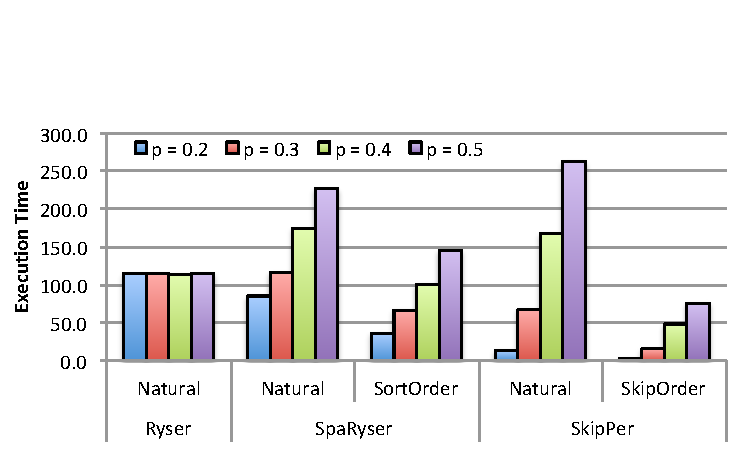
\includegraphics[width=0.5\linewidth]{fig2}
    \qquad
    \scalebox{0.92}{
 \begin{tabular}[b]{l | r | rr | rr} 
 	&	\sc{Ryser}	&	\multicolumn{2}{|c}{\sc{SpaRyser}}		&	\multicolumn{2}{|c}{\sc{SkipPer}}	\\
	$p$&	Nat.	&	Nat.	&	Ord	&	Nat.	&	Ord.	\\\hline
0.2	&	0.01	&	0.28	&	0.29	&	0.32	&	0.39	\\
0.3	&	0.01	&	0.10	&	0.23	&	0.20	&	0.33	\\
 0.4	&	0.00	&	0.05	&	0.12	&	0.15	&	0.25	\\
 0.5	&	0.01	&	0.08	&	0.01	&	0.09	&	0.18	\\
 \multicolumn{6}{c}{}\\
  \multicolumn{6}{c}{}\\								
 \end{tabular}
 }
 \captionlistentry[table]{A table beside a figure}
    \captionsetup{labelformat=andtable}
    \caption{The execution times (in seconds) of the algorithms for $n = 32$ and $p = \{0.2, 0.3, 0.4, 0.5\}$ of the algorithms {\sc{Ryser}}, {\sc{SpaRyser}} and {\sc{SkipPer}} with and without ordering on randomly generated matrices~(left) and variations of coefficient for the execution times on five matrices used for each ($n, p$) pair~(right). The bars labeled as {\em{Natural}} show the executions where no ordering is applied to the given matrix and the natural order is used. }
    \label{firstfig}
     \end{figure}

 The algorithm {\sc{SkipPer}} improves the performance drastically; although it can perform much worse when the matrix is unordered, with {\sc{SkipOrder}} its performance improves significantly. Even for $p = 0.5$,  {\sc{SkipPer}} is $1.6\times$ faster than {\sc{Ryser}}. For $p = 0.2$, the speedup is around $40\times$. The speedups of {\sc{SkipPer}} with {\sc{SkipOrd}} over {\sc{Ryser}} with different $n$ and $p$ values are given in Table~\ref{tab:seq}.

\begin{table}[!htbp]
\centering
\scalebox{0.93}{
\begin{tabular}{l  | rrrr}
& \multicolumn{4}{c}{$p$} \\\hline
$n$ & $0.2$ &  $0.3$ &  $0.4$ & $0.5$\\\hline
32 &40.1$\times$  & 10.8$\times$ & 2.5$\times$ & 1.6$\times$\\
34 &119.7$\times$ & 11.2$\times$ & 3.8$\times$ & 1.6$\times$ \\
36 &140.9$\times$ & 13.2$\times$ & 4.2$\times$ & 1.6$\times$ \\
 \end{tabular}
 }
 \caption{Speedups of to {\sc{SkipPer}} over {\sc{Ryser}} with different $n$ and $p$ values.}
 \label{tab:seq}
 \end{table}

Table~\ref{tab:all} compares the algorithms in a pairwise manner for $n = 32$ and $p = \{0.2, 0.3, 0.4, 0.5\}$. As described above, we generated $20$ matrices for $n = 32$ with different $p$ values. To compare two algorithms, for each matrix, we divide the execution time of former to that of the latter and we report the averages of these $20$ values in the table. As the results confirm, {\sc{SkipPer}} performs much better than the other two algorithms. Furthermore, {\sc{SortOrd}} is a better ordering for {\sc{SpaRyser}}, and {\sc{SkipOrd}} yields around $20\%$ better performance for {\sc{SkipPer}} compared to {\sc{SortOrd}}. Although better orderings may still exist, these two observations show the validity of the rationale behind the orderings designed specially for {\sc{SpaRyser}} and {\sc{SkipPer}}. 

\begin{table}[!htbp]
\centering
\scalebox{0.93}{
\begin{tabular}{ll  | r  | rrr  | rrr}
 	&&	\sc{Ryser}	&	\multicolumn{3}{|c}{\sc{SpaRyser}} &	\multicolumn{3}{|c}{\sc{SkipPer}}	\\\hline
	&  &		&		&	\sc{Sort}	&	\sc{Skip}	&		&	\sc{Sort}	&	\sc{Skip}\\
Algorithm	& Ordering &	Nat.	&	Nat.	&	\sc{Ord}	&	\sc{Ord}	& Nat.		&	\sc{Ord}	&	\sc{Ord}	\\\hline
\sc{Ryser} & Natural		&	1.0	&-		&-		&-		&	-	&-		&-		\\\hline
	& Natural & 	0.9	&	1.0	&-		&-		&-		&-		&-		\\
\sc{SpaRyser} & \sc{SortOrd}	&	1.8	&	1.9	&	1.0	&-		&-		&-		&-		\\
 & \sc{SkipOrd}	&	1.7	&	1.8	&	0.9	&	1.0	&-		&-		&-		\\\hline
	& Natural &	2.9	&	2.6	&	1.3	&	1.4	&	1.0	&-		&-		\\
\sc{SkipPer} & \sc{SortOrd}	&	11.0	&	9.5	&	4.7	&	5.0	&	3.4	&	1.0	&-		\\
 & \sc{SkipOrd}	&	13.7	&	12.1	&	5.9	&	6.3	&	4.1	&	1.2	&	1.0	\\
 \end{tabular}
 }
 \vspace*{1ex}
 \caption{Pairwise performance comparison of the algorithms for $n = 32$. For each row, the performances are normalized w.r.t. to the algorithm whose name is given 
 in the leftmost column at that row. Each value in the table is the average of normalized execution times for $20$ different executions since we have four different $p$ values and five matrices for each $p$.}
 \label{tab:all}
 \end{table}
   
We evaluate the performance of the approach described in the previous section to parallelize {\sc{SkipPer}}. We use $16$ threads with coarse grain parallelism by dividing the iteration space of length $2^{n-1} - 1$ to $16$. We also measured the performance when much smaller chunks are created and assigned by dynamic scheduling. We present the speedup results with $16$ chunks, i.e., static scheduling~(columns $10$--$13$) and $512$ chunks with dynamic scheduling~(columns $6$--$9$) in Table~\ref{tab:speedup}. The results confirm that with smaller chunks, one can have almost linear speedup, i.e., between $14.4$ and $15.2$ with $\tau = 16$ threads. However, especially for sparser matrices, where the number of skipped iterations can greatly vary, the parallel efficiency is low with static scheduling. Columns $2$-$5$ in the table present the speedups w.r.t. sequential {\sc{Ryser}} when $\tau = 16$ threads is used. Overall, parallel {\sc{SkipPer}} is around $600\times$--$2000\times$ faster than{\sc{Ryser}} and the speedups decrease with decreasing sparsity.  
 
 \begin{table}[!htbp]
 \centering
 \scalebox{0.93}{
 \begin{tabular}{l | rrrr | rrrr || rrrr}
& \multicolumn{4}{c}{Speedup w.r.t. seq.} &   \multicolumn{4}{|c||}{Speedup w.r.t. seq.} &   \multicolumn{4}{c}{Speedup w.r.t. seq.}\\
& \multicolumn{4}{c}{\sc{Ryser}} &   \multicolumn{4}{|c||}{\sc{SkipPer}-\sc{SkipOrd}} &   \multicolumn{4}{c}{\sc{SkipPer}-\sc{SkipOrd}}\\
& \multicolumn{4}{c}{(dyn., \#chunks = 512)} &   \multicolumn{4}{|c||}{(dyn., \#chunks = 512)} &   \multicolumn{4}{c}{(stat., \#chunks = 16)}\\
& \multicolumn{4}{c}{$p$} &   \multicolumn{4}{|c||}{$p$ }&   \multicolumn{4}{c}{$p$}\\
$n$ 	&$0.2$	&$0.3$	&$0.4$	&$0.5$	&$0.2$	&$0.3$	&$0.4$	&$0.5$ &$0.2$	&$0.3$	&$0.4$	&$0.5$\\\hline
32	&605	&161	&37.2	&23.7	&15.2	&15.1	&14.8	&15.3 &6.6	&10.3	&11.1	&11.7\\
34	&1790	&172	&57.4	&24.4	&14.4	&15.2	&15.2	&15.5 &6.1	&9.8	&9.8	&10.7 \\
36	&2050	&180	&49.2	&24.2	&14.6	&15.0	&15.5	&15.6 &6.8	&9.0	&10.6	&13.7 \\
 \end{tabular}
 }
 \vspace*{1ex}
 \caption{Speedups of parallel {\sc{SkipPer}}-{\sc{SkipOrd}} with $\tau = 16$ threads: columns $2$--$5$ show the improvement with dynamic scheduling w.r.t. the traditional {\sc{Ryser}}. Columns $6$--$9$ present the speedups w.r.t. the sequential algorithm. To show the benefits of dynamic scheduling, columns $10$--$13$ show the speedup values with static scheduling.}
 \label{tab:speedup}
 \end{table}
 
 \subsection{Experiments with Real-Life Matrices}
 
In addition to synthetic matrices, we used five real-life matrices to further evaluate the performance of the proposed algorithms. The properties of the matrices and the results of the experiments are given in Table~\ref{tab:real}. 
For each matrix, we used the decomposition technique~\eqref{eq:expand} in~\cite{forbert03, liang06} to recursively decompose the matrix into two. The decomposition is performed until there is no row/column having less than $5$ nonzeros or $n \leq 32$. Each algorithm is run with a 30-minute time limit and computed the permanent of as many sub-matrices as they can. For each algorithm $alg$, Table~\ref{tab:real} reports the number of sub-matrices $alg$ processes, the number of sub-matrices on which $alg$ is the fastest, and $alg$'s average relative performance with respect to that of {\sc{SkipPer-SkipOrd}}. The relative performance is computed only over the matrices processed by $alg$~(since {\sc{SkipPer}} is the fastest algorithm and the time limit is the same for all the algorithms, we have its execution times on these matrices). We consider an algorithm as best for a matrix if its execution time does not exceed $1.05\times$ of the minimum permanent computation time for that matrix. As the table shows, although there are matrices for which {\sc{SpaRyser}} is better than {\sc{SkipPer}}, i.e., $6$ sub-matrices for {\tt c100} and one sub-matrix for {\tt chesapeake}, the average performance of {\sc{SkipPer}} is much better than the other two algorithms. 

In addition to the individual performances of {\sc{Ryser}}, {\sc{SpaRyser}} and {\sc{SkipPer}}, the last two columns of the table present the speedups for  {\sc{SkipPer}} both with static and dynamic scheduling and  $\tau = 16$ w.r.t. sequential {\sc{SkipPer}}. The results confirm the previous experiments; static scheduling can fail to balance the load distribution whereas parallelization with dynamic scheduling yields close to linear speedups. 
 
 \begin{table}[!htbp]
 \centering
 \scalebox{0.90} {
 \begin{tabular} {l | rr | rrr | rrr | rrr | r | r}
   		&  \multicolumn{2}{c|}{}  &   \multicolumn{3}{c|}{}  & \multicolumn{3}{c|}{{}}  &  \multicolumn{3}{c|}{} &  \multicolumn{2}{c}{{\sc{SkipPer-SkipOrd}}} \\
  		&  \multicolumn{2}{c|}{Prop.}  &   \multicolumn{3}{c|}{{\sc{Ryser}}} &  \multicolumn{3}{c|}{{\sc{SpaRyser-SortOrd}}}  &  \multicolumn{3}{c|}{{\sc{SkipPer-SkipOrd}}} &\multicolumn{2}{c}{$\tau = 16$, speedup}\\\hline
 Matrix 		& $n$ & $nnz$ &  Solved & Best & Perf.   &  Solved & Best & Perf. &  Solved & Best & Perf. & static & dynamic \\\hline
 {\tt bfwb62}   	& 62 & 202 & 15 & - & 37.8 & 49 & - & 11.7 & 520& 520 & 1.0& 7.1$\times$&14.7$\times$\\	
 {\tt  c100}		& 100 & 300 & 15 & - & 4.3 & 38 & 14 &  1.2 & 42 & 36 & 1.0& 14.9$\times$& 15.9$\times$\\
 {\tt  cage5}	& 37 & 233 & 10 & - & 22.2 & 10 & - & 6.2 & 10 & 10 & 1.0& 6.7$\times$&13.6$\times$\\
 {\tt  chesapeake}	& 39 & 340 & 15 & - & 11.8 & 44 & 7 & 5.5 & 84 & 83 & 1.0 & 5.6$\times$& 14.8$\times$\\	
 {\tt  will57	}	& 57 & 281 & 15 & -  & 69.2 & 64 & - &  13.4 & 609 & 609 & 1.0& 8.3$\times$& 14.7$\times$
 \end{tabular}
 }
 \vspace{1ex}
 \caption{The table shows the number of matrices processed, number of matrices with the fastest execution time, and the relative performance with respect to {\sc{SkipPer}} for each algorithm. For each row, several sub-matrices are generated by using the decomposition given in Eq.~\ref{eq:expand}. The last two columns present the speedup values for {\sc{SkipPer}} with static and dynamic scheduling, respectively.}
 \label{tab:real}
 \end{table}
 
\section{Conclusion and Future Work} \label{sec:conc}

In this work, we proposed parallel algorithms for efficient computation of permanents of sparse matrices. Compared to the original algorithm {\sc{Ryser}}, we obtained around $2000\times$ speedups for matrices with high sparsity. The proposed techniques can be used to improve the performance of the existing solutions in the literature since at one point they almost all use {\sc{Ryser}}. The best algorithm {\sc{SkipPer}} uses Gray skipping whose impact heavily depends on the nonzero pattern in the matrix. Although we proposed {\sc{SkipOrder}} and showed its effectiveness empirically, it can be an interesting future work to generate the best ordering that enables the algorithm to cover the iteration space with the fewest number of skips and yield the best theoretical complexity. In addition, one can also combine our work with the technique proposed by Servedio and Wan~\cite{servedio05} which adds a row/column to the original matrix to obtain an augmented matrix to encounter many zero terms during {\sc{Ryser}}. 

Another possible research avenue is parallelizing {\sc{Skipper}} on many-core devices such as GPUs. We expect that the problem will be much harder since balancing the load is not an easy task with thousands of cores. However, the Gray skipping technique as well as the proposed ordering technique can be easily adopted since they create independent tasks with possibly varying but small computational loads. 

%bibliography style

\newpage
\begin{thebibliography}{10}

\bibitem{nijenhuis78}
Nijenhuis A and Wilf HS.
\newblock {\em Combinatorial Algorithms}.
\newblock Academic Press, 1978.

\bibitem{yue13}
Yue B, Liang H, and Bai F.
\newblock Improved algorithms for permanent and permanental polynomial of
  sparse graph.
\newblock {\em MATCH}, 69:831--842, 01 2013.

\bibitem{bax08}
Bax E and Franklin J.
\newblock A permanent algorithm with exp[$\omega(n^{1/3}/2\ln{n})$] expected
  speedup for 0-1 matrices.
\newblock {\em Algorithmica}, 32:157--162, 01 2008.

\bibitem{kilic07}
K{\i}l{\i}\c{c} E and Tas\c{c}{\i} D.
\newblock On the permanents of some tridiagonal matrices with applications to
  the {F}ibonacci and {L}ucas numbers.
\newblock {\em Rocky Mountain J. Math.}, 37:1953--1969, 2007.

\bibitem{dufosse18}
Dufoss{\'e} F, Kaya K, Panagiotas I, and U{\c c}ar B.
\newblock {Scaling matrices and counting the perfect matchings in graphs}.
\newblock Research Report RR-9161, {Inria Grenoble Rh{\^o}ne-Alpes}, March
  2018.

\bibitem{forbert03}
Forbert H and Marx D.
\newblock Calculation of the permanent of a sparse positive matrix.
\newblock {\em Computer Physics Communications}, 150(3):267 -- 273, 2003.

\bibitem{liang06}
Liang H, Huang S, and Bai F.
\newblock A hybrid algorithm for computing permanents of sparse matrices.
\newblock {\em Applied Mathematics and Computation}, 172(2):708 -- 716, 2006.
\newblock Special issue for The Beijing-HK Scientific Computing Meetings.

\bibitem{minc84}
Minc H and Marcus M.
\newblock {\em Permanents}.
\newblock Encyclopedia of Mathematics and its Applications. Cambridge
  University Press, 1984.

\bibitem{ryser63}
Ryser HJ.
\newblock {\em Combinatorial Mathematics}.
\newblock Mathematical Association of America, 1963.

\bibitem{Wang2012ALB}
Wang L, Liang H, Bai F, and Huo Y.
\newblock A load balancing strategy for parallel computation of sparse
  permanents.
\newblock {\em Numerical Lin. Alg. with Applic.}, 19:1017--1030, 2012.

\bibitem{valiant79}
Valiant LG.
\newblock The complexity of computing the permanent.
\newblock {\em Theoretical Computer Science}, 8(2):189 -- 201, 1979.

\bibitem{narahara13}
Narahara M, Tamaki K, and Yamada R.
\newblock Application of permanents of square matrices for {DNA} identification
  in multiple-fatality cases.
\newblock {\em BMC Genetics}, 14(1):72, Aug 2013.

\bibitem{balakrishnan07}
Balakrishnan N.
\newblock Permanents, order statistics, outliers, and robustness.
\newblock {\em Revista Matematica Complutense, 2007}, 20, 03 2007.

\bibitem{mittal01}
Mittal RC and Al-Kurdi A.
\newblock Efficient computation of the permanent of a sparse matrix.
\newblock {\em International Journal of Computer Mathematics}, 77(2):189--199,
  2001.

\bibitem{aaronson11}
Aaronson S and Arkhipov A.
\newblock The computational complexity of linear optics, 2010.

\bibitem{servedio05}
Servedio S and Wan A.
\newblock Computing sparse permanents faster.
\newblock {\em Information Processing Letters}, 96(3):89--92, 11 2005.

\end{thebibliography}

\end{document}
